%PRECEDENTE: variabile-complessa
\chapter{L'integrale complesso}

Siamo abituati ad effettuare integrali su linee; abbiamo quindi bisogno di definire una curva in $\C$:

\begin{definizione}

Una curva è una funzione $\gamma:[a;b]\subset\R\to\C$ continua e differenziabile con continuità (cioè esiste il vettore tangente alla curva in ogni punto). La curva ha un verso di percorrenza, che va da $\gamma(a)$ a $\gamma(b)$.

Una curva si dice chiusa se si verifica che $\gamma(a)=\gamma(b)$; se la curva è chiusa e non ha avvolgimenti, cioè se la curva non ha ulteriori intersezioni oltre all'inizio e alla fine della stessa, è detta curva di Jordan.
\end{definizione}
Esempi:
\begin{itemize}
\item Un segmento nel piano complesso, di estremi $z_1$ e $z_2$ è una curva con parametrizzazione $\gamma(t)=z_1+(z_2-z_1)t$, con t$\in$[0;1]. Il vettore tangente è $\dot{\gamma}(t)=z_2-z_1$, cioè è sempre costante in ogni punto della curva.
Un'altra parametrizzazione del segmento è $\tilde{\gamma}(t)=z_1+(z_2-z_1)t^2$, con $t\in[0;1]$; in questo caso, il vettore tangente è $\dot{\tilde{\gamma}}(t)=2t(z_2-z_1)$, cioè non è costante.
\item Una circonferenza di centro $z_0$ e raggio $\rho$ è parametrizzata da $\gamma(\theta)=z_0+\rho e^{i \theta}$, con $\theta \in[0;2\pi]$; il vettore tangente alla curva è $\dot{\gamma}(\theta)=i \rho e^{i \theta}$, cioè è il vettore $\rho e^{i\theta}$ ruotato di $\frac{\pi}{2}$
\end{itemize}
Indicheremo con $\tilde{\gamma}(t)$ o con $-\gamma$ la parametrizzazione che percorre in senso opposto la curva $\gamma$, cioè $\tilde{\gamma}(t)=\gamma(a+b-t):[a;b]\to\C$.
\\
Adesso possiamo introdurre il concetto di integrale nel piano complesso:
\begin{definizione}
Sia $\gamma$ un cammino nel piano complesso con parametrizzazione $\gamma[a;b]\to\C$ differenziabile con continuità; sia f una funzione della variabile z continua sulla curva $\gamma$. Definiamo integrale di una funzione $f$ sulla curva $\gamma$ la quantità:
$$\int_\gamma f(z)dz=\int_a ^b f(\gamma(t))\dot{\gamma}(t)dt=\int_a ^b (u(\gamma_1,\gamma_2)+iv(\gamma_1,\gamma_2))(\dot{\gamma_1}+i\dot{\gamma_2})dt$$ L'integrale di una funzione nel piano complesso è quindi la somma di quattro integrali di Riemann.
\end{definizione}
Introduciamo due importanti disuguaglianze; sia $f:[a;b]\to\C$ continua. Allora:
\begin{itemize}
\item $\left|\int_a^b f(t)dt\right|\leq\int_a^b \left|f(t)\right| dt$. \\ Dimostriamo questo fatto; abbiamo che $\int_a^b f(t)dt$ è un numero complesso, quindi possiamo scriverlo come $\int_a^b f(t)dt=\left|\int_a^b f(t)dt\right|e^{i\theta}$. Possiamo riscrivere l'equazione come $\left|\int_a^b f(t)dt\right|=$ $=e^{-i\theta}\int_a^b f(t)dt=\int_a^b e^{-i\theta} f(t)dt$. Dato che $e^{-i\theta}f(t)$ è un numero reale, posso prenderne la parte reale; ma $Re(z)\leq |z|$, e quindi abbiamo che $\left|\int_a^b f(t)dt\right|=\int_a^b Re(e^{-i\theta} f(t))dt\leq$  $\leq \int_a^b |f(t)|dt$.$_{\Box}$ 
\end{itemize}

\begin{osservazione}
Gli operatori $Re$ e $Im$ possono essere portati dentro e fuori l'integrale liberamente; infatti:
%$$Re\left(\int_a^b f(t)dt\right)=Re\left(\int_a^b(u+iv)dt\right)=Re\left(\int_a^bu \, dt\right)+Re\left(\int_a^b iv \, dt\right)=\int_a^bu \, dt=\int_a^b Re(f(t))dt$$%
$$Re \int_a^b f(t)dt=Re \int_a^b(u+iv)d=Re \int_a^bu \, dt +Re \int_a^b iv \, dt =\int_a^bu \, dt=\int_a^b Re(f(t))dt$$
\end{osservazione}

\begin{itemize}
\item \textbf{Disuguaglianza di Darboux}: $\left|\int_{\gamma} f(z) dz\right| \leq L[\gamma] \, \sup_{z \in \gamma} |f(z)|$, dove $L[\gamma]$ rappresenta la lunghezza della curva $\gamma$. Dimostriamo questa disuguaglianza: 
$$\left|\int_{\gamma} f(t) dt\right|=\left|\int_a ^b f(\gamma(t))\dot{\gamma}(t)dt\right| \leq \int_a ^b |f(\gamma(t))| \, |\dot{\gamma}(t)|dt \leq$$
$$\leq \sup_{t \in [0;1]} |f(\gamma(t))|\, \int_a ^b \sqrt{\dot{\gamma_1 ^2}+\dot{\gamma_2 ^2}}dt=\sup_{t \in [0;1]} |f(\gamma(t))| \, L[\gamma] \leq L[\gamma] \sup_{z \in \gamma} |f(z)|$$
\end{itemize}
Un'altra proprietà utile da tenere a mente è la seguente:
$$\int_{-\gamma} f(z) dz=-\int_{\gamma} f(z) dz$$

\section{La funzione primitiva}

Introduciamo ora il concetto di primitiva per una funzione complessa:
\begin{definizione}
Sia $f:D \subset \C \to \C$ una funzione continua su D. La funzione F si dice primitiva di f in D se F è olomorfa su D e vale che $F'(z)=f(z)$ $\forall z \in D$.
\end{definizione}
Se F è primitiva di f, abbiamo che:
$$\int_{\gamma}f(z)dz=\int_a ^b f(\gamma(t))\dot{\gamma}(t)dt=\int_a ^b F'(\gamma(t))\dot{\gamma}(t)dt=\int_a ^b \frac{d}{dt}(F(\gamma(t)))dt=F(\gamma(b))-F(\gamma(a))$$ Oltretutto, abbiamo che, se $\gamma$ è chiusa, allora l'integrale risulta nullo.

Sia $f(z)=z^n$; la sua primitiva è $F(z)=\frac{z^{n+1}}{n+1}$ per $n \neq -1$. Poniamo $D\equiv \C \backslash \{(0;0)\}$. Prendiamo poi la circonferenza centrata nell'origine di raggio 1, parametrizzata da $\gamma(\theta)=e^{i \theta}$; l'integrale della funzione $z^n$ sulla curva $\gamma$ è:
$$\int_{\gamma} z^n dz=\int_0 ^{2\pi} e^{i n \theta} i e^{i \theta} d\theta=i \int_0 ^{2\pi} e^{i (n+1) \theta} d\theta=$$
$$=i \int_0 ^{2\pi} \left[cos((n+1)\theta)+isen((n+1)\theta)\right] d\theta= \left\{
  \begin{array}{l l}
    0 & \quad \text{se $n \neq -1$}\\
    2 \pi i & \quad \text{se $n=-1$}
  \end{array} \right.$$

La funzione $\frac{1}{z}$ è olomorfa in $\C \backslash \{(0;0)\}$, La sua primitiva è $Log(z)$, olomorfa in $\C \backslash \{(x;0) : x \in (0;+\infty]\}$. Se come cammino prendiamo la circonferenza precedentemente utilizzata, il valore dell'integrale non è nullo, perchè il cammino scelto attraversa la zona in cui la curva non è olomorfa. Prendiamo la curva $\gamma_{\epsilon}$, cioè l'arco di circonferenza che unisce i punti $-1-i\epsilon$ e $-1+i\epsilon$ senza attraversare il semiasse negativo delle ascisse, e calcoliamo l'integrale della funzione $\frac{1}{z}$ su di essa:
$$\int_{\gamma_{\epsilon}}=Log(-1+i\epsilon)-Log(-1-i\epsilon) \to i\pi -(-i\pi)=2i\pi \text{ per } \epsilon \to 0$$
Infine, introduciamo una funzione che traduce analiticamente questa situazione, la funzione indice:
\begin{definizione}
Sia $\gamma$ un cammino chiuso e differenziabile con continuità (a tratti). Chiamiamo funzione indice di $\gamma$ rispetto a $z_0$ (con $z_0 \notin \gamma$) la funzione 
$$Ind(\gamma,z_0)=\int_{\gamma} \frac{1}{z-z_0} \frac{dz}{2 \pi i}$$
\end{definizione}

La funzione indice restituisce il numero di avvolgimenti della curva $\gamma$ intorno al punto $z_0$. Se la curva è una curva di Jordan,  allora la funzione indice restituirà il valore 1; se la curva invece ha ulteriori intersezioni, possiamo immaginare di dividere la curva in tante curve di Jordan senza riutilizzare due volte lo stesso tratto di curva. In questo modo, possiamo facilmente contare il numero di avvolgimenti, che equivale a contare il numero di attraversamenti del taglio della funzione logaritmo principale.

\begin{figure}[h!]
  \centering
    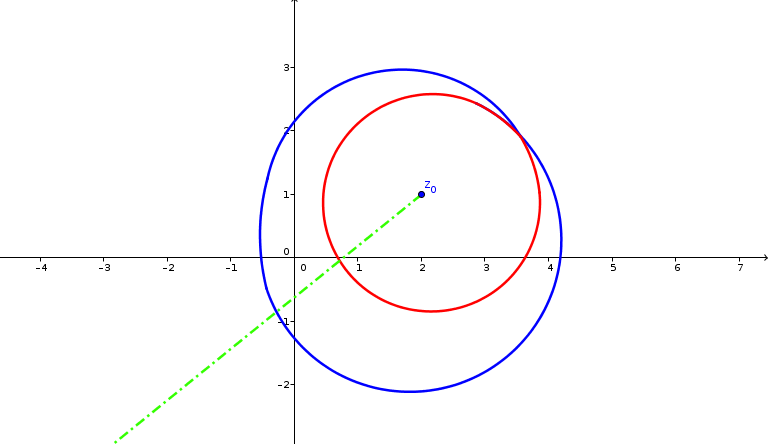
\includegraphics[width=0.75 \textwidth]{immagini/indice.png}
\end{figure}
\begin{teorema}
Sia $f$ una funzione continua sul dominio D. Sono equivalenti le seguenti affermazioni:
\begin{enumerate}
\item $\int_{z_1}^{z_2} f(z)dz$ non dipende dal cammino $\gamma$ che unisce $z_1$ a $z_2$ in $\C$
\item $\exists \, \int_{\gamma} f(z)dz \, \forall$ cammino chiuso $\gamma$ in D (differenziabile con continuità a tratti)
\item $\exists$ una primitiva $F$ (funzione olomorfa su D tale che $F'=f$ su D)
\end{enumerate}
\end{teorema}
\begin{proof}
E' banale dimostrare le implicazioni $1) \implies 2)$ e $3) \implies 1),2)$. Dimostriamo l'implicazione $1) \implies 3)$.\\Chiamiamo $F(z)=\int_{z_0}^{z} f(z')dz'$; valutiamo $F(z+h)=F(z)+\int_{z}^{z+h} f(z')dz'$, dove $h\in \C$. \\Parametrizzando il segmento, otteniamo:
$$\gamma(t)=z+th \text{ e } \dot{\gamma}(t)=h$$
$$F(z+h)=F(z)+h \int_{0}^{1} f(z+th)dt \implies$$
$$\implies \frac{F(z+h)-F(z)}{h}-f(z)=\int_{0}^{1} f(z+th)dt-f(z)=\int_{0}^{1} f(z+th)-f(z)dt$$
Sappiamo che $\forall \, \epsilon >0 \, \exists \, \delta_{\epsilon}: \, |f(z+h)-f(z)|<\epsilon \, \forall \, h: \, |h|<\delta_{\epsilon}$; quindi:
$$\left|\frac{F(z+h)-F(z)}{h}-f(z)\right| = \left|\int_{0}^{1} f(z+th)-f(z)dt\right| \leq \int_{0}^{1} |f(z+th)-f(z)|dt \leq \epsilon $$
La frazione al primo membro della prima equazione tende a $f(z)$ per $h \to 0$, cioè la prima frazione va a 0; dato che la seconda diseguaglianza vale $\forall \, \epsilon > 0$, abbiamo la tesi.
\end{proof}

La funzione inversione $\frac{1}{z}$  è una funzione olomorfa su $\C \backslash \{0\}$; la sua primitiva è il logaritmo principale $Log(z)$, che è olomorfa su $\C \backslash \{(x;0) \, : \, x<0\}$. \\ Data una curva chiusa $\gamma$, abbiamo visto la funzione indice $Ind(\gamma,z)=\frac{1}{2i \pi} \int_{\gamma} \frac{dz'}{z'-z}$ che restituisce il numero di avvolgimenti della curva intorno al punto $z$ ($\notin \gamma$); se la curva circonda $z$, attraverserà il taglio, altrimenti la funzione diventa semplicemente l'integrale lungo una curva chiusa (che dà come risultato 0). Operativamente, basta contare gli attraversamenti del taglio da parte della curva $\gamma$: possiamo avere attraversamenti ''dall'alto verso il basso'' e ''dal basso verso l'alto''; i primi corrispondono ad avvolgimenti antiorari, il cui contributo è di $2i \pi$ (+1 per la funzione indice), i secondi ad avvolgimenti in senso antiorario, il cui contributo è $-2i \pi$ (-1 per la funzione indice). \\ La richiesta che il punto z non appartenga alla curva è dovuta al fatto che non è definito l'indice di un punto su una curva.
\\
Introduciamo ora un importante teorema, il teorema di Cauchy-Goursat:

\begin{teorema}(di Cauchy-Goursat)\\Sia $f$ una funzione olomorfa su un dominio $\mathcal{D}$; sia $\mathfrak{R}$ un rettangolo contenuto in $\mathcal{D}$; allora:
$$\int_{\partial \mathfrak{R}} f(z)dz=0$$
\end{teorema}
\begin{proof}
Dividiamo il rettangolo $\mathfrak{R}$ in quattro sottorettangoli che ereditano l'orientazione del bordo dal rettangolo di partenza; chiameremo questi quattro rettangoli prima generazione di rettangoli. Valutando l'integrale sulla frontiera di questi rettangoli, notiamo che i contributi sui lati in comune si annullano a vicenda, perchè l'orientazione è opposta; possiamo quindi scrivere:
$$\mathcal{I}=\int_{\partial \mathfrak{R}} f(z)dz=\sum_{i=1} ^4 \int_{\partial \mathfrak{R}_{1i}} f(z)dz$$
$$|\mathcal{I}| \leq \sum_{i=1} ^4 \left|\int_{\partial \mathfrak{R}_{1i}} f(z)dz \right| \leq 4|\mathcal{I}_1|$$ dove $\mathcal{I}_1$ è il rettangolo che ha modulo di valore massimo; dividendo questo rettangolo in altri quattro rettangoli e iterando le precedenti operazioni, otteniamo:
$$|\mathcal{I}| \leq 4|\mathcal{I}_1| \leq 4 \sum_{i=1} ^4\left|\int_{\partial \mathfrak{R}_{2i}} f(z)dz \right| \leq 4^2|\mathcal{I}_2| \leq \dots \leq 4^n |\mathcal{I}_n|$$
\\
Sia $L$ la diagonale del rettangolo $\mathfrak{R}$; quando dividiamo il rettangolo, la diagonale del rettangolo di generazione $n$ risulta essere $\frac{L}{2^n}$. \\ Abbiamo che $\mathfrak{R} \supset \mathfrak{R}_1 \supset \mathfrak{R}_2 \supset \dots \supset \mathfrak{R}_n$; per $n \to +\infty$, si ha che  $A_{\mathfrak{R}_n} \to 0$. \\Per un teorema dovuto a Cantor, sappiamo che esiste un punto $a$ tale che $\bigcap_{k=1} ^{+ \infty} \mathfrak{R}_k =\{a\}$.\\$f$ è una funzione olomorfa; allora possiamo scrivere $\frac{f(z)-f(a)}{z-a}$ attraverso la somma $f'(a)+r(z,a)$, dove $r(z,a)$ è tale che $|r(z,a)| \to 0$ quando $z \to a$. Quindi l'integrale calcolato sul rettangolo $\mathcal{I}_n$ (cioè il rettangolo avente area maggiore fra quelli di $n$-esima generazione) risulta essere:
$$\mathcal{I}_n= \int_{\partial \mathfrak{R}_n} f(z)dz = \int_{\partial \mathfrak{R}_n} [f(a)+f'(a)(z-a) + r(z,a)(z-a)]dz$$ A questo punto, dividiamo l'integrale secondo le somme; ci si accorge  che i primi due membri hanno contributi nulli, perchè sia $f(a)$ sia $(z-a)$ hanno primitiva e, dato che stiamo integrando su un cammino chiuso, per il teorema precedente abbiamo che l'integrale è nullo. Rimane quindi solo l'ultimo membro; passando ai moduli, otteniamo:
$$|\mathcal{I}_n|\leq \int_{\partial \mathfrak{R}_n} |r(z,a)| \, |(z-a)| \, dz \leq \epsilon \frac{L}{2^n} \, 4 \frac{L}{2^n}$$ dove $4 \frac{L}{2^n}$ maggiora il cammino; sostituendo nella relazione $|\mathcal{I}|=4^n |\mathcal{I}_n|$, otteniamo che $|\mathcal{I}| \leq 4 L^2 \epsilon$ e, per l'arbitrarietà di $\epsilon$, abbiamo dimostrato la tesi.
\end{proof}
\begin{teorema}
Sia $f$ una funzione continua su un dominio $\mathcal{D}$ e olomorfa su $\mathcal{D} \backslash \{a\}$; sia $\mathfrak{R}$ un rettangolo contenuto in $\mathcal{D}$; allora vale ancora il teorema dei rettangoli, cioè $\int_{\partial \mathfrak{R}} f(z)dz=0$.
\end{teorema}
\begin{proof}
Se il punto è all'interno del rettangolo, lo isoliamo con delle strisce verticali e orizzontali; è evidente che possiamo scrivere il rettangolo $\mathfrak{R}$ come la somma dei rettangoli $\mathfrak{R}_i$, e vale ancora la legge di cancellazione dei tratti in comune; quindi $\mathcal{I}=\sum_i \int_{\partial \mathfrak{R}_i} f(z)dz$. \\ Di questa sommatoria sopravvive soltanto il rettangolino contenente il punto $a$, cioè $\mathcal{I}=\int_{\partial \mathfrak{r}} f(z)dz$. A questo punto, possiamo scrivere che $|\mathcal{I}| \leq \sup_{z \in \mathfrak{r}} |f(z)| L(\mathfrak{r})$, dove $L(\mathfrak{r})$ è il perimetro del rettangolino. \\ Giocando sul fatto che possiamo prendere il rettangolo $\mathfrak{r}$ piccolo a piacere, facciamo tendere a zero il perimetro e quindi otteniamo la tesi.\\Se invece il punto è sul bordo, procediamo in maniera analoga; cambia solo la ''divisione'' del rettangolo (in questo caso, avremo che una delle due strisce è a ridosso del lato al quale appartiene $a$).
\end{proof}

%SUCCESSIVO: funzioni-intere